\documentclass[UTF8,11pt,oneside]{ctexart}

\def\articletitle{中东狂买中国电子产品,要求生产组装起运均在中国}
\usepackage{CJKfntef}
\usepackage{float}

\usepackage{geometry}
\geometry{a4paper,left=2cm,right=2cm,top=2cm,bottom=1cm}

\usepackage{graphicx}

\usepackage{hyperref}
\hypersetup{colorlinks=true, linkcolor=red}

\linespread{1.6}

\usepackage{fancyhdr}
\usepackage{ifthen}
\pagestyle{fancy}
\fancyhf{}
\setlength{\headheight}{14pt}
\fancyhead[R]{\ifthenelse{\value{page}>1}{\thepage}{}}
\fancyhead[C]{\ifthenelse{\value{page}>1}{\articletitle}{}}
\renewcommand\headrulewidth{0pt}

\usepackage{tcolorbox}
\tcbuselibrary{skins}

\newcommand{\zd}[1]{\textbf{\textcolor[RGB]{123,12,0}{#1}}} % 重点

\newcommand{\yinyong}[1]{% 引用
    \begin{tcolorbox}[enhanced,
        frame hidden, interior hidden,
        before skip = 5mm, left skip=10mm,
        borderline west={5pt}{0pt}{gray!50}]
        #1
    \end{tcolorbox}
}

\newcommand{\xhx}[1]{%下划线(模拟微信中的划线功能,用于标注我个人认为的文章中精彩的地方)
    \CJKunderline*[thickness=1.5pt, format=\color[RGB]{84,216,140}]{#1}
}

\newcommand{\biaoti}[1]{% 标题
    \section*{#1}
}

\newcommand{\SetSectionType} {
    \ctexset{
        section={
            number = \chinese{section},
            aftername={、},
            format=\Large\bfseries,
        }
    }
}



\begin{document}

\begin{center}
    \LARGE{\articletitle\footnotemark}
\end{center}
\footnotetext{
    原文出自公众号“远方青木”的文章 《\href{https://mp.weixin.qq.com/s/PSeaaQxFSNww4wswQcLEaw}{\articletitle}》
}

以色列在同时引爆黎巴嫩5000寻呼机(台湾品牌)之后,又引爆了黎巴嫩大量对讲机(日本制造),共造成数千人伤亡,医护 、平民、真主党被无差别大量杀伤。

不仅有数百人下体被炸烂,还有数百人双眼被炸伤,黎巴嫩全国医生都被紧急召集,24小时工作来救治伤员。

黎巴嫩眼科专家埃利亚斯·瓦拉克对记者说:

\yinyong{
    “我一晚上摘除的坏死眼球,数量比我之前整个职业生涯中摘除的加起来还要多。”

    过去的24小时就像一场“噩梦”,超过60\%至70\%的伤者被摘除了一只眼睛。

    真的非常难受。大多数伤者都是二十几岁的年轻小伙子,有些病人不得不摘除双眼,我一辈子没见过那样的场面。
}

\zd{打开伤者的纱布后,记者看到的是一个又一个空洞洞的眼窟窿,这一幕不仅深深震撼了记者,也震撼了整个阿拉伯世界。}

\begin{figure}[H]
    \centering
    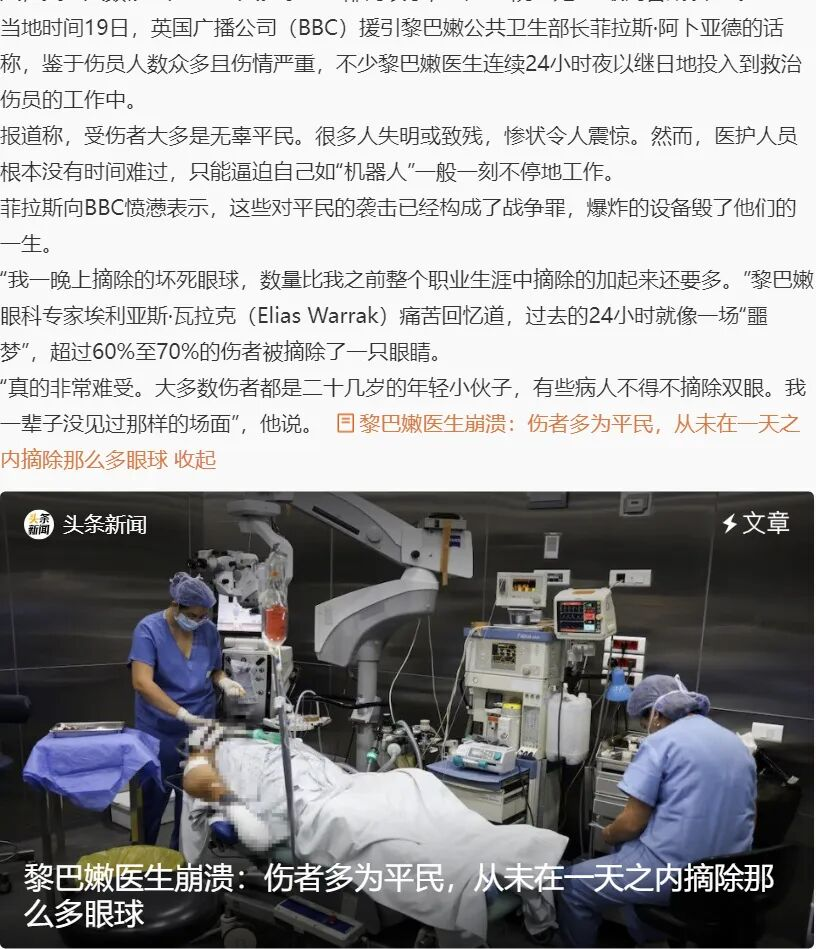
\includegraphics[width=12cm]{2024-09-21-001.jpg}
\end{figure}

与以色列为敌的可不止黎巴嫩,整个阿拉伯世界都和以色列为敌,今天以色列能这么炸黎巴嫩人,明天就可以炸任何一个阿拉伯人。

而且这种无差别袭击太可怕了,是无差别杀戮,富人穷人一起杀,而且就算中东富人们把自己用的电子产品彻底检查,但万一自家仆人所用的手机突然爆炸时飞溅的碎片射到自己眼睛里呢?

这次被送进黎巴嫩的伤者,很多并不是电子产品的携带者,只是爆炸时恰好站在电子产品携带者旁边而已。

就算给仆人以及身边工作人员统一配备电子产品,中东王子和富人们总是要出门的,如果本国每一个群众身上携带的电子产品都可能变成炸弹,让自己随时有双目失明的风险,这日子简直没法过了。

英国每日邮报还特地发了篇文章,标题是“\zd{俄罗斯可以让数百万部iPhone毫无预警的爆炸}”,把黎巴嫩受伤民众的照片和普京头像放在了一起。

\begin{figure}[H]
    \centering
    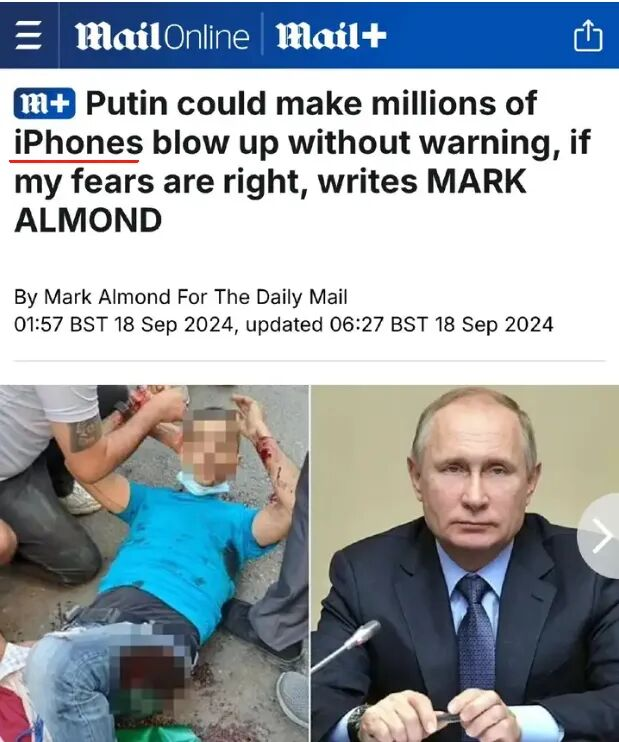
\includegraphics[width=12cm]{2024-09-21-002.jpg}
\end{figure}

英国人蔫坏蔫坏的,苹果手机不是英国造的,俄罗斯倒霉是英国喜闻乐见的,所以才炮制出这样的新闻,我估计苹果总裁库克撕了英国每日邮报的心都有了。

但英国每日邮报毕竟代表了英国洋大人的意见,俄罗斯是不是能让数百万iPhone毫无预警的爆炸这件事存疑,但按英国人的说法,毫无疑问的是数百万iPhone可以做到毫无预警爆炸。

\zd{有没有让俄罗斯人害怕不好说,但中东人肯定是害怕了。}

在X平台和油管上,中东头像的人已经在相关帖子下刷屏了,意见高度一致,那就是绝对不能再买西方的电子产品了。

完全可以理解他们为什么这么想,要是我们自己被这么炸一下,同样也不会有安全感的。

\zd{随后中国有人贴出了自家工厂收到的中东客户询价邮件,和以往询价邮件不同的是,这次额外添加的条件是产品所有零部件必须均为中国制造,同时生产组装也必须都在中国,然后还要求必须是中国起运。}

\begin{figure}[H]
    \centering
    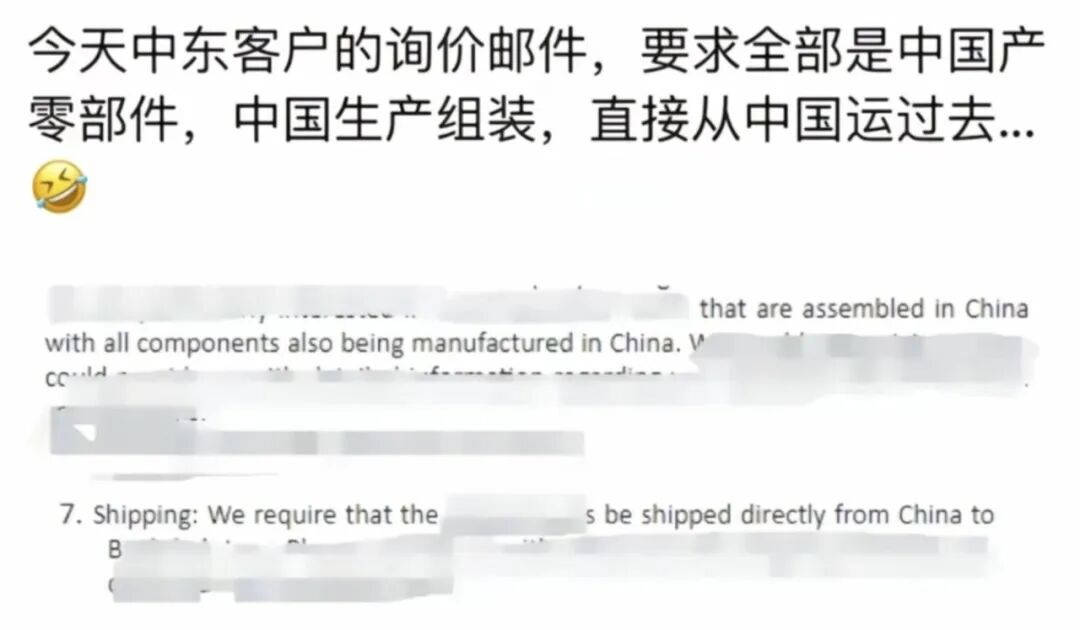
\includegraphics[width=12cm]{2024-09-21-003.jpg}
\end{figure}

\zd{Made In China到底代表高端货还是低端货,这个争论到今天有了答案,Made In China代表了安全,代表了肯定不会爆炸。}

\xhx{安全不一定可以代表高端,但不安全的东西肯定代表不了高端。}

中东人这波被数千同胞惨状给吓出来的心理应激反应远超预期,不仅发到中国工厂的询价邮件要求产品从头到脚都必须中国造,还有中东人要求连运货的船都必须是中国的,同时上面的船员也必须是中国籍,确保整个交付流程没有一丝一毫被西方人接触到的可能性。

\begin{figure}[H]
    \centering
    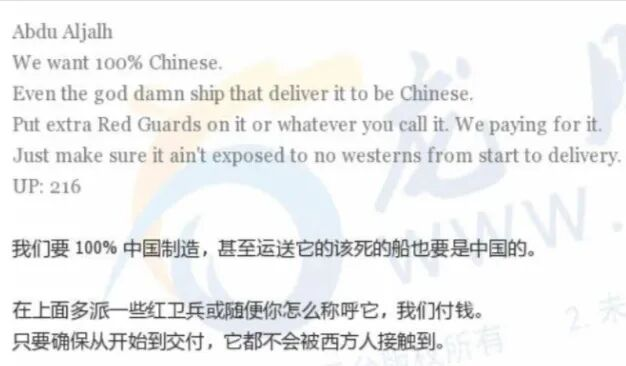
\includegraphics[width=12cm]{2024-09-21-004.jpg}
\end{figure}

\zd{国际贸易做了这么多年,这种要求还是头一次见。}

\zd{目前涌过来的第一波中东订单潮,主要是贴身电子产品,什么蓝牙设备穿戴设备都在此列,离身体越近的中东人越害怕。}

都知道西方电子产品一定会搞窃听,但窃听这种事只要做好首脑人物的防范就好了,万万没想到西方的电子产品会针对成千上万的普通民众搞爆炸。

这就没法重点防范了,本国也造不出来必须外购,那保证全民安全的办法就只剩了一个了,也就是向中国采购,使用纯中国造产品,中东国家想要保证本国百姓安全,在目前的世界格局下没有其他选项了。

中东人并不是都亲华的,相反亲西方的人特别多,哪怕被以色列打了那么多年都有大量的中东人亲西方,因为慕强是人之本性,而在过去的一个多世纪里强者和西方是等价词。

就算是黎巴嫩,国内也有很多人是亲西方的。

但这轮以色列的炸弹把这些亲西方的中东人都给炸醒了,因为这些炸弹可不认人,不会因为你的态度是亲西方的就不炸你了,更不能保证你亲人的安全。

如今的中东人无论态度是否亲西方,贴身的电子产品都不敢用西方货了,中国造的产品特别抢手。

\zd{有些东西,人教人教不会,事教人一教就会。}

\begin{figure}[H]
    \centering
    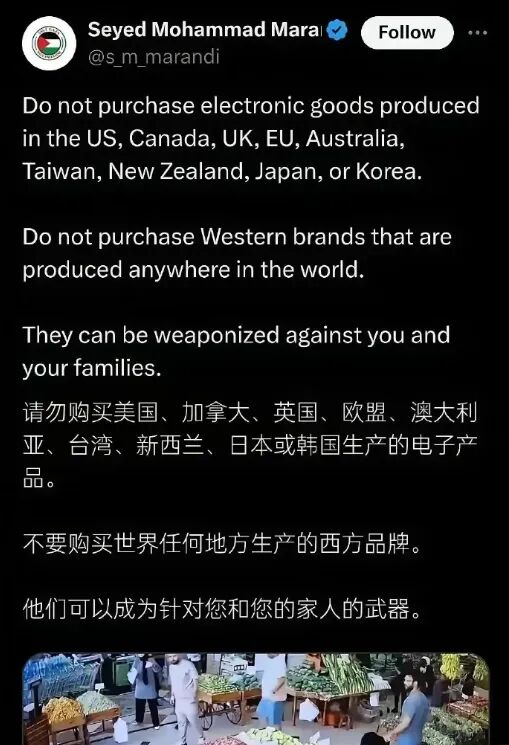
\includegraphics[width=11cm]{2024-09-21-005.jpg}
\end{figure}

\zd{为了打入中东市场,中国的电子产品这么多年来花了大量心血和资金进行宣传,效果不及以色列这一炸的零头。}

欧美封锁俄罗斯后,等于把俄罗斯市场拱手让给了中国,有人说俄罗斯才1.4亿人,GDP只相当于一个广东省。

但他们没说的是广东省的GDP单拎出来排世界前十,也就是俄罗斯这种级别的市场全球只有十个。

如今以色列这一炸,又把中东市场最肥的一块拱手送给了中国。

中东有4亿人口,而且什么都缺就是不缺钱,全球皆知“头顶一块布,全球我最富”,除了被欧美长期狂轰滥炸的那几个中东国家稍微困难点,其他都是富得流油。

就算论人均,中东都是富国,一个客户很难同时拥有中东和穷这两个标签,这是一个人口和财富规模都仅次于欧盟的市场。

整个欧盟也才4亿人口,而且人均GDP也就比中东强一截而已,中东只是工业特别弱才显得国家很弱,但论“钱”这个东西,真不缺。

中国正好是工业特别强,只缺“钱”这个东西,能拿下中东市场对中国来说属于完美互补。

而且除中东这一圈富国之外,面对这种无差别杀伤民众的电子产品袭击。

阿尔及利亚、埃塞俄比亚、安哥拉、贝宁、博茨瓦纳、布基纳法索、布隆迪、几内亚、多哥、厄立特里亚、佛得角、冈比亚、刚果(布)、刚果(金)、吉布提、几内亚、几内亚比绍、加纳、加蓬、津巴布韦、喀麦隆、科摩罗、科特迪瓦、肯尼亚、莱索托、利比里亚、利比亚、卢旺达、马达加斯加、马拉维、马里、毛里求斯、毛里塔尼亚、摩洛哥、莫桑比克、纳米比亚、南非、南苏丹、尼日尔、尼日利亚、塞拉利昂、塞内加尔、塞舌尔、圣多美和普林西比、斯威士兰、苏丹、索马里、坦桑尼亚、突尼斯、乌干达、赞比亚、乍得、中非、哈萨克斯坦、吉尔吉斯斯坦、塔吉克斯坦、乌兹别克斯坦、土库曼斯坦 以及中南半岛国家、东南亚国家、拉丁美洲国家等等。

他们会怎么想?虽然这些国家的老百姓暂时不担心被欧美的电子产品炸,但再购买欧美电子产品的时候,心里会不会嘀咕一下?

\zd{所谓的国际社会,看到黎巴嫩人民被电子产品大规模炸伤的时候心里一点不害怕的,可能就只有这么几个国家了。}

\begin{figure}[H]
    \centering
    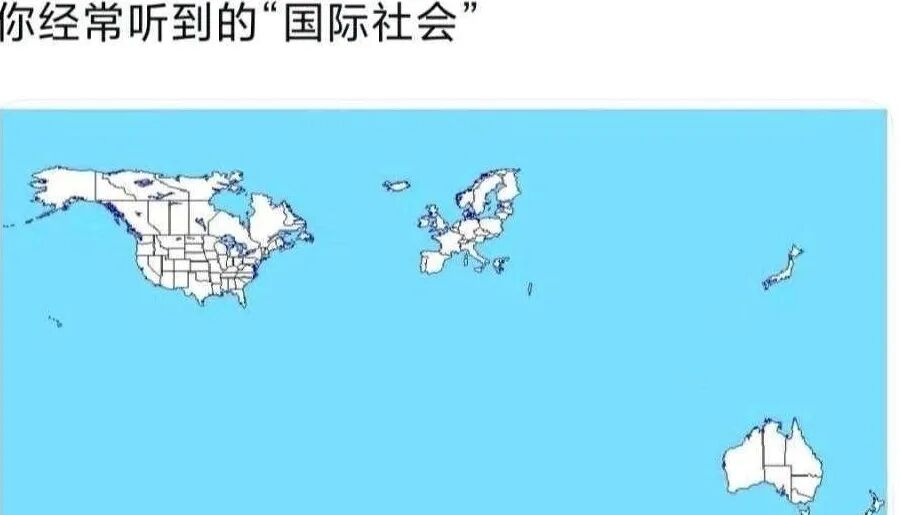
\includegraphics[width=12cm]{2024-09-21-006.jpg}
\end{figure}

\zd{当今世界有三圣,足以配享太庙的那种。}

前有乌克兰泽连斯基泽圣,以一人之力振兴中国东北,并将俄罗斯市场送给了我们。

中有阿根廷米莱米圣,量阿根廷之物力结中国之外汇,以一人之力让中国的老百姓吃上了低价的优质牛肉。

后有以色列内塔尼亚胡内圣,以一人之力匡扶整个中国的电子产业。

用来炸黎巴嫩老百姓的电子产品,还一个是台湾品牌,一个是日本品牌,内圣实在是太贴心了,在大力促进中国产品销售的时候还顺手精准打击了台湾和日本产品的销售。

把民用电子产品改造为杀人炸弹,这种事相当于西方产品的洛水之誓,全球范围内政治和经济都是分开的,政治上吵的再凶,经济上都是该怎么买就怎么买,最多也就加个关税而已,其他一律市场经济。

万万没想到有人会在民用电子产品里放炸弹。

洛水当年是很神圣的,但司马懿违反洛水之誓后,数千年的时间里没人敢再对着洛水发誓了。

公知不是老说信用这东西,一旦失去,就很难再回来了嘛。

说的一点都没错,不过失去的是西方产品的信用。

正常情况下中国产品想在中东打造出信用度,最低需要几十年时间,当年欧美崛起的时候也都是这么过来的,他们的商品建立如今的霸主地位都不是一朝一夕之功,想取代旧体系是很难的,很多商品的采购都有巨大的惯性。

中国产品眼热中东市场很久了,但饭要一口口的吃,市场要一点点的开拓,急不得,只能慢慢来。

没想到如今人在家中坐,市场天上来。

真正意义上的躺赢。

\begin{figure}[H]
    \centering
    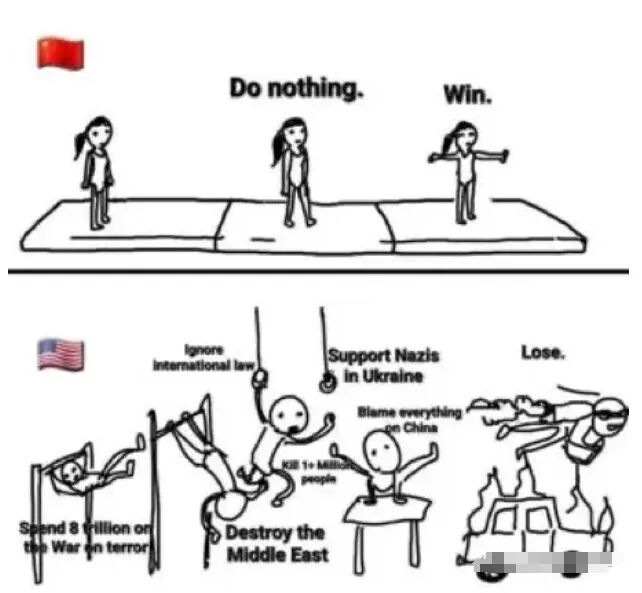
\includegraphics[width=12cm]{2024-09-21-007.jpg}
\end{figure}

这就是国运,标准的国运,再厉害的谋士都算不出来对手能使出如此蠢的招数。

怪不得十几天前,国足打日本的时候给踢了个0比7,全国都不理解为什么能输这么多,前所未有的大惨败。

\zd{十天后以色列引爆黎巴嫩5000寻呼机之后我们明白了,原来国足这是在平衡国运啊。}

\zd{这几天真的是委屈国足了,下次再接再厉踢个0比10。}

\end{document}

